\documentclass[a4paper,12pt]{article}
\usepackage{CJKutf8}
\usepackage{amsthm}
\usepackage{amsmath}
\usepackage{amssymb}
\usepackage{geometry}
\usepackage{graphicx}
\usepackage{array}
\usepackage{subfigure}
\usepackage{gbt7714}
\usepackage{appendix}
\usepackage{listings}
\usepackage{xcolor}
\usepackage{tikz}
\usepackage{float}
\usepackage{tcolorbox}
\usepackage[colorlinks,linkcolor=blue,anchorcolor=blue,citecolor=blue,]{hyperref}
\usepackage{bookmark}
\lstset{
    language=c++,
    basicstyle=\ttfamily,
    keywordstyle=\color{blue},
    numbers=left,
    numberstyle={\ttfamily\scriptsize\color{red!60!black!60!white}},
    numbersep=5pt,
    columns=flexible,
    breaklines=true,
    keywordstyle    =   \color{blue},
    keywordstyle    =   [2] \color{teal},
    stringstyle     =   \color{magenta},
    commentstyle    =   \color{red}\ttfamily,
}


%\bibliographystyle{gbt7714-numerical}
% 边距
\geometry{left=1.0cm,right=1.0cm,top=3.0cm,bottom=3.0cm}
\renewcommand{\figurename}{图}
\begin{document}
\begin{CJK}{UTF8}{song}
\title{图生成与分解器}
\author{李子龙\\\small 电子信息与电气工程学院\\\small 518070910095 F1903301}
\date{2020 年 12 月 24 日}
\maketitle
\normalsize

\begin{tcolorbox}
    Copyright \copyright\ 2020 by LogCreative, All Rights Reserved.
    
    To learn more about the author, please visit \href{https://github.com/LogCreative}{https://github.com/LogCreative}.

    (LC) No. 0211
\end{tcolorbox}

\section{问题重述}

\begin{enumerate}
    \item 开发一个图自动生成器
    
    随机生成一个有向图,将图放置到指定文件中,每一行如下格式
    \begin{itemize}
        \item $\langle$节点编号$\rangle$:节点
        \item $\langle$出发节点编号,结束节点编号,权重$\rangle$:有向边
    \end{itemize}

    \item 开发一个图分解器
    \begin{itemize}
        \item 分割图文件
        \begin{itemize}
            \item 将上述图分为若干子图,每个子图中节点数不大于$n$。
            \item $A$图分割后,每个子图可以用单独的文件保存:如 \texttt{A1,A2,A3},$\cdots$
            \item 令子图之间的交互(即能够跨越子图边界的边)权重之和最小,我们将挑选若干自动生成的图,对比大家生成的权重之和值。在结果正确的前提下,计算权重之和越小,分数越高。
        \end{itemize}
        \item 优化子图存储
        
        上述图分割算法导致分割成的多个子图之间存在重复的节点,请设计一个方法,使
        \begin{itemize}
            \item 多个子图文件中分别载入程序后,不存在重复的节点
            \item 每个子图可以最多增加一个虚节点(如子图的文件名),代表外界(即其他子图)对该子图的引用
            \item 设计一个算法,将多个子图合并及删除虚节点后,检查与原图$A$一致。输出分割边的权重和。
        \end{itemize}
        \item 子图上算法
        \begin{itemize}
            \item 指定一个点,列出计算所有经有向边可达的节点
            \item 指定两个点,输出最短路径
            \item 如果指定的节点不存在,报错即可
        \end{itemize}
    \end{itemize}
\end{enumerate}


\section{公共类 \texttt{GraphCommon}}

在开始的无 UI 编译时期,存储为同一个公共类 \texttt{GraphCommon},后面因为需要使用全局的非静态变量,将头文件分离。该类的完整版本还是请看 \texttt{GraphDecomp.h} 中的相关定义。

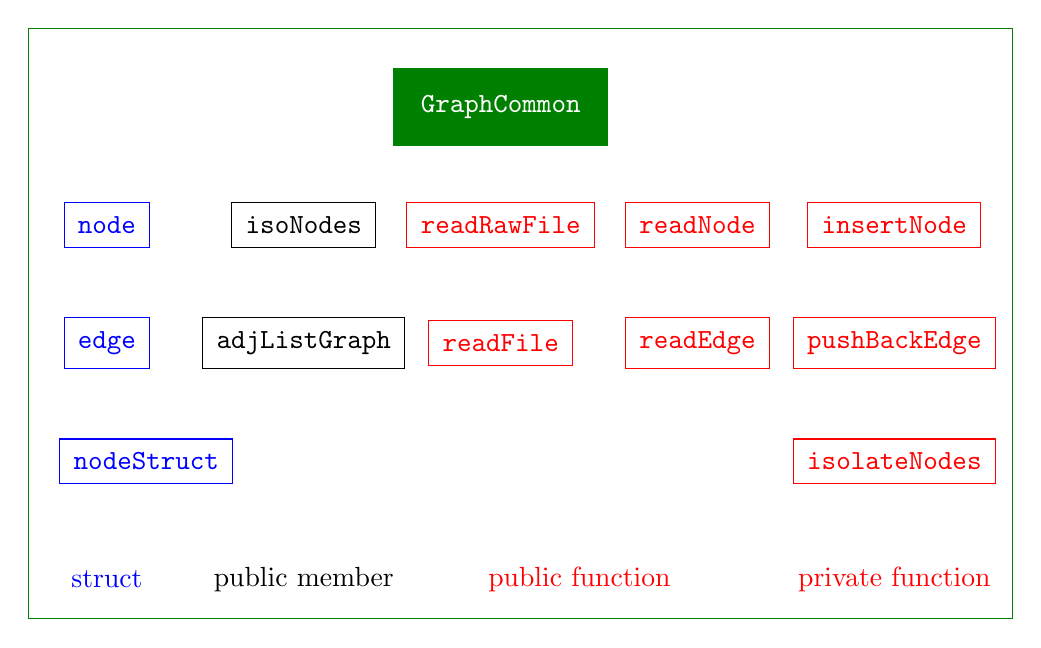
\begin{tikzpicture}
\tikzstyle{class} = [font=\ttfamily\bfseries,color=white,fill=green!50!black,inner sep=10];
\tikzstyle{struct} = [font=\ttfamily\bfseries,color=blue,draw=blue, inner sep = 5];
\tikzstyle{member} = [font=\ttfamily,draw, inner sep=5]
\tikzstyle{function} = [font=\ttfamily\bfseries,color=red,draw=red, inner sep = 5];
\node [class] at (-2,3.5) {GraphCommon};
\node [struct] at (-7,2) {node};
\node [struct] at (-7,0.5) {edge};
\node [struct] at (-6.5,-1) {nodeStruct};
\node [member] at (-4.5,2) {isoNodes};
\node [member] at (-4.5,0.5) {adjListGraph};
\node [function] at (-2,0.5) {readFile};
\node [function] at (-2,2) {readRawFile};
\node [function] at (0.5,2) {readNode};
\node [function] at (0.5,0.5) {readEdge};
\node [function] at (3,2) {insertNode};
\node [function] at (3,0.5) {pushBackEdge};
\node [function] at (3,-1) {isolateNodes};
\draw [green!50!black]  (-8,4.5) rectangle (4.5,-3);
\node [blue] at (-7,-2.5) {struct};
\node at (-4.5,-2.5) {public member};
\node [red] at (-1,-2.5) {public function};
\node [red] at (3,-2.5) {private function};
\end{tikzpicture}

\subsection{结构体}

该类定义了三个小结构体:
\begin{itemize}
    \item 节点类 \texttt{node}
    \item 有向边类 \texttt{edge}
    \item 节点结构 \texttt{nodeStruct}(用于计算邻接矩阵)
\end{itemize}

前两个都重载了输入输出运算符,以符合目标格式。

\begin{table}[H]
    \begin{tabular}{cll}{}
        &输入&输出\\
        \hline
        \texttt{node}&$\langle$\texttt{P1}$\rangle$&$\langle$1$\rangle$\\
        \texttt{edge}&$\langle$\texttt{P1 P2 2.0}$\rangle$&$\langle$\texttt{1,2,2.0}$\rangle$\\
        \hline
    \end{tabular}
\end{table}


前缀符号以及分割符可以在后面调整。值得一提的是,优化后子图的虚边定义为如下的格式:
\begin{verbatim}
<起始点,虚点符号,<文件名.终止节点,权重>>
<1,-1,<O1.2,2.0>>
\end{verbatim}
在本程序中,\texttt{-1}被定义虚节点符号。

节点结构中定义了三个成员:
\begin{itemize}
    \item 邻接矩阵边存储
    \item 邻接矩阵列数值
    \item 节点发出边总权重
\end{itemize}

并通过两个私有函数同步更新这些数值。

\subsection{公共成员}

该类定义了两个公共成员:
\begin{itemize}
    \item \texttt{set<int> isoNodes} 包含了所有的孤立节点(isolated nodes),也就是完全不连通的部分。
    \item \texttt{map<int, vector<edge>> adjListGraph},邻接表图,仅包含连通部分节点,对于有些连通节点可能为发出空边的集合,即 \texttt{adjListGraph[node] = vector<edge>({});}。
\end{itemize}

\subsection{公共函数}

该类定义了四个公共函数。
\begin{itemize}
    \item \texttt{readNode} 通过输入文本流读取明确定义的节点信息
    \item \texttt{readEdge} 通过文本流读取有向边的信息。
    \item \texttt{readFile} 通过文本流读取文件信息。
    \item \texttt{readRawFile} 通过文本流读取特定格式的文件信息。
\end{itemize}

\subsection{私有函数}

该类定义了三个私有函数。
\begin{itemize}
    \item \texttt{insertNode} 插入节点,包含了对虚节点的检查机制。
    \item \texttt{pushBackEdge} 向邻接表插入边,也包含了对节点是否为虚节点的转换检查机制。
    \item \texttt{isolateNodes} 将 \texttt{readNode} 后的集合去除根据 \texttt{readEdge} 所读取的连接边点,变为孤立节点的集合。
\end{itemize}


\section{图生成器 \texttt{GraphGen}}

图生成器的类 \texttt{GraphGen} 是 \texttt{GraphCommonGen} 的派生类。

本程序的图生成器有几个参数需要设置:

\begin{itemize}
\item
  \textbf{节点类型} \texttt{nodeType}:\texttt{continuous}连续编号的,
  \texttt{discrete}离散的。
\item
  边生成类型 \texttt{edgeType}:\texttt{Tree}树(不含环路),
  \texttt{Graph}图(带有环路)。
\item
  \textbf{连通图类型} \texttt{isoType}:\texttt{Single} 单个连通图,
  \texttt{Multi} 多个连通图。
\item
  \textbf{节点编号增长量}
  \texttt{MAX\_INCREASEMENT}:在离散编号模式下,每次生成一个节点都会增长一个数字,这个数字不会超过最大增长量
  。
\item
  \textbf{最大孩子数}
  \texttt{MAX\_CHILD}:每个节点的发出有向边个数不会超过最大孩子数 。
\item
  \textbf{最大连通子图数}
  \texttt{MAX\_ISOGRAPH}:在多个连通图生成模式下,每个图的连通子图数不会超过最大连通子图数。
\item
  \textbf{节点行数占比}
  \texttt{Node\ /\ Lines}:在新文件模式下,仍然会生成随机个数的节点数,但是只输出占比量的节点行数,其余为有向边的行。
\end{itemize}

该程序将会根据上述参数,递增而随机地生成节点编号。然后通过层序遍历生成各个边,如果没有环路的限制,则有可能随机到一个环路节点上去。

随机数采用下面的代码生成:

\begin{lstlisting}
srand((unsigned)time(0)*(++gseed));
return 1.0 * rand() / RAND_MAX;	
\end{lstlisting}

当然,这种方式依然不是特别特别随机,但已经足够。



\end{CJK}
\end{document}